\documentclass[uplatex,dvipdfmx,a4paper,11pt]{jsarticle}

\usepackage{url}
\usepackage[dvipdfmx]{hyperref}

\usepackage[top=25mm,bottom=25mm,left=25mm,right=25mm]{geometry}

\usepackage{array}
\usepackage{tabularx}
\usepackage{booktabs}
\usepackage{enumitem}
\usepackage{graphicx}
\usepackage{longtable}

\setlength{\parindent}{0pt}
\setlength{\parskip}{0.6em}

\usepackage{titlesec}
\titleformat{\section}
  {\normalfont\Large\bfseries}{\thesection.}{0.6em}{}
\titleformat{\subsection}
  {\normalfont\large\bfseries}{\thesubsection}{0.6em}{}
\titlespacing*{\section}{0pt}{1.2em}{0.6em}
\titlespacing*{\subsection}{0pt}{1.0em}{0.4em}

\newcommand{\sectionrule}{\par\medskip\noindent\rule{\linewidth}{0.6pt}\par\medskip}

\renewcommand{\labelitemi}{\textbullet}
\renewcommand{\labelitemii}{\textopenbullet}
\setlist[itemize]{leftmargin=1.6em,itemsep=0.1em,topsep=0.2em}
\setlist[enumerate]{leftmargin=2.0em,itemsep=0.1em,topsep=0.2em}

\providecommand{\textopenbullet}{\ensuremath{\circ}}


\begin{document}


{\LARGE\bfseries 作業ログ}\par\bigskip

報告者：佐藤涼菜

報告日：6月16日

プロジェクト名：マジカル☆観覧車

\sectionrule


\section{進捗サマリー（要約）}

\begin{itemize}
  \item 全体進捗率：60[％]
  \item マイルストーン達成状況：一部未達（指揮デバイスの筐体実装が最終段階）
  \item 主要成果：
    \begin{itemize}
      \item {指揮デバイスの筐体（段ボール製）の制作がほぼ完成（No.2112）}
      \item {基盤に設置したスライド式可変抵抗器・ボタン・センサ類を筐体へ配置（No.2112）}
      \item {タクトスイッチの動作確認用プログラム（button\_test）の作成・検証（No.2112）}
    \end{itemize}
  \item 重大課題（影響度：高）：
    \begin{itemize}
      \item {指揮デバイスの筐体（No.2112）はほぼ完成したが，最終固定が残っている．また，1機のスライド式可変抵抗器のはんだ付け設置不良が6/10に判明し，再はんだ付けの修正が必要であった．}
    \end{itemize}
\end{itemize}

\sectionrule


\section{作業ログ（詳細トラッキング）}

\subsection{作業ログ}

\renewcommand{\arraystretch}{1.2}

\small

\begin{longtable}{|c|p{2.2cm}|c|c|c|c|p{2.4cm}|p{3.1cm}|}
\caption{作業ログ} \\
\hline
No. & 作業項目 & 開始日 & 予定完了日 & 状態 & 進捗率 & 依存関係・ブロッカー & コメント \\
\hline
\endfirsthead

\hline
No. & 作業項目 & 開始日 & 予定完了日 & 状態 & 進捗率 & 依存関係・ブロッカー & コメント \\
\hline
\endhead

\hline
\multicolumn{8}{r}{次ページへ続く} \\
\hline
\endfoot

\hline
\endlastfoot

2112 &
本体・センサの実装 &
5/24 &
6/16 &
進行中 &
90\% &
無 &
段ボール筐体の制作がほぼ完成．基盤設置済の可変抵抗器・ボタン・センサ類を筐体へ配置．残りは最終固定のみ． \\
\hline

2113 &
BPM・音量変化機構の実装 &
5/29 &
6/16 &
進行中 &
85\% &
通信部の結合待ち &
可変抵抗器から読み取った値を5段階にして出力する処理は実装・検証済．残りはUDP送信（通信部）の結合． \\
\hline

- &
作業ログの記入 &
6/10 &
6/16 &
完了 &
100\% &
無 &
特になし． \\
\hline



\end{longtable}


\subsection{日ごとの作業ログ}


    \renewcommand{\arraystretch}{1.2}

    \small

    \begin{longtable}{|c|c|p{2.4cm}|c|c|c|c|p{3.8cm}|}
    \caption{日ごとの作業ログ} \\
    \hline
    日付 & No. & 作業項目 & 時間 & 開始時の状態 & 終了時の状態 & 進捗率 & コメント \\
    \hline
    \endfirsthead

    \hline
    日付 & No. & 作業項目 & 時間 & 開始時の状態 & 終了時の状態 & 進捗率 & コメント \\
    \hline
    \endhead

    \hline
    \multicolumn{8}{r}{次ページへ続く} \\
    \hline
    \endfoot

    \hline
    \endlastfoot

    6/10 & 2112 & 本体・センサの実装 & 2h &
    進行中 &
    進行中 &
    75\% &
    タクトスイッチの動作確認用プログラム（button\_test）を作成し，押下検知を確認．1機のスライド式可変抵抗器のはんだ付け設置不良が判明し，再はんだ付けの修正を実施．基盤設置済の可変抵抗器を筐体へ仮配置． \\
    \hline

    6/11 & 2112 & 本体・センサの実装 & 1.5h &
    進行中 &
    進行中 &
    80\% &
    段ボール筐体のスライダー用開口部・ボタン穴の加工を実施． \\
    \hline

    6/12 & 2112 & 本体・センサの実装 & 2h &
    進行中 &
    進行中 &
    85\% &
    基盤・可変抵抗器・ボタン・センサ類を筐体内部に固定し，配線を整理． \\
    \hline

    6/13 & 2112 & 本体・センサの実装 & 1.5h &
    進行中 &
    進行中 &
    90\% &
    筐体上部の蓋を加工し，スライダー・ボタンの操作面を成形． \\
    \hline

    6/14 & 2112 & 本体・センサの実装 & 1h &
    進行中 &
    進行中 &
    88\% &
    筐体の外観を整え，各操作部が干渉なく動作することを確認． \\
    \hline

    6/15 & 2112 & 本体・センサの実装 & 1h &
    進行中 &
    進行中 &
    90\% &
    筐体の最終調整を実施し，ほぼ完成．残りは最終固定のみ． \\
    \hline

    6/16 & - & 作業ログの記入 & 1h &
    未着手 &
    完了 &
    100\% &
    特になし． \\

    \end{longtable}

\sectionrule

\section{計画時のGCと現在のGC}

最終計画書に記載された計画段階のガントチャート(GC)を図\ref{fig:gant1}に示す．

\begin{figure}[htbp]
    \centering
    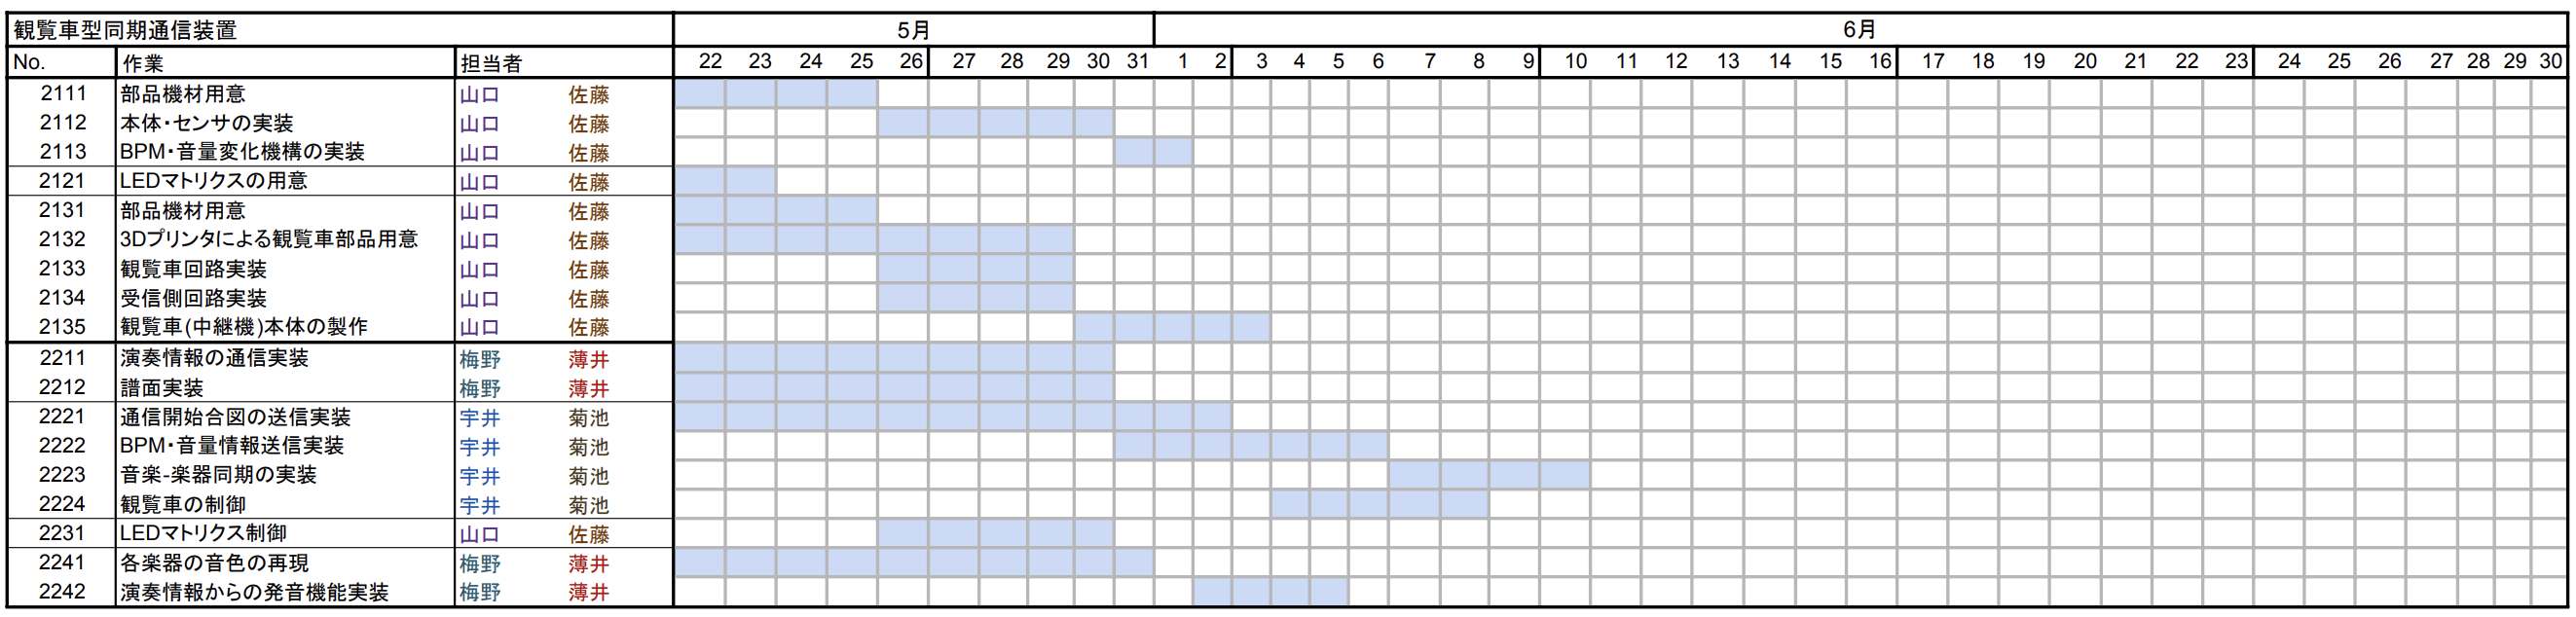
\includegraphics[width=0.8\columnwidth]{gant1.png}
    \caption{計画段階のガントチャート}
    \label{fig:gant1}
\end{figure}

次に，現在のGCを図\ref{fig:gant7}（実装フェーズ）および図\ref{fig:gant8}（テストフェーズ）に示す．達成した項目は緑色で塗られている．

\begin{figure}[htbp]
    \centering
    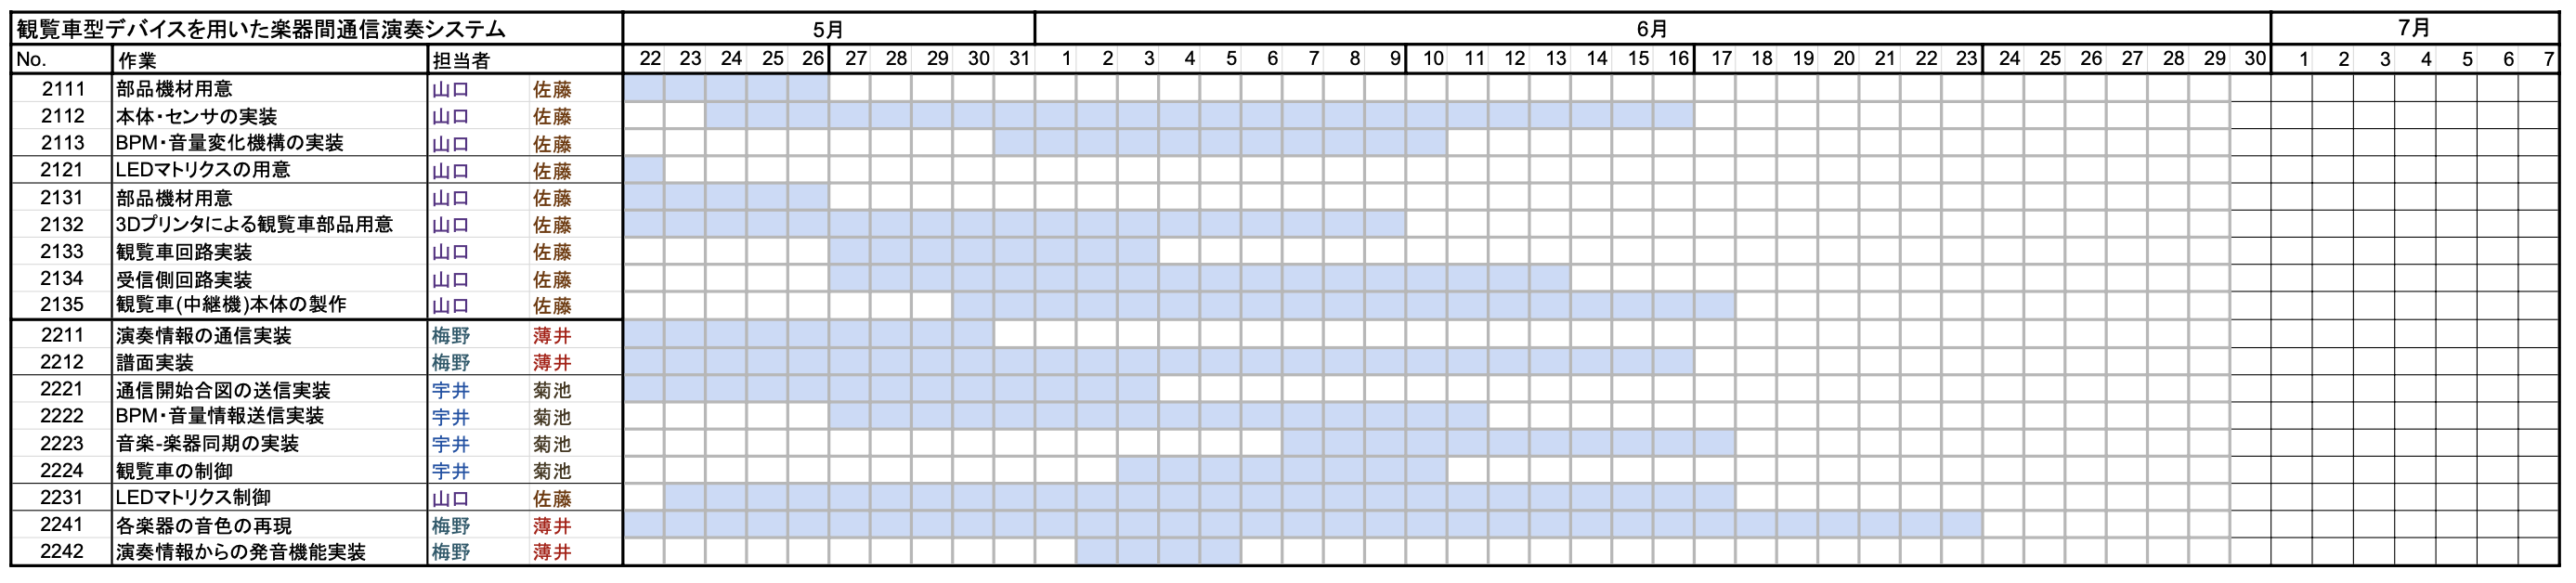
\includegraphics[width=0.9\columnwidth]{gant7.png}
    \caption{現在のガントチャート（実装フェーズ）}
    \label{fig:gant7}
\end{figure}

\begin{figure}[htbp]
    \centering
    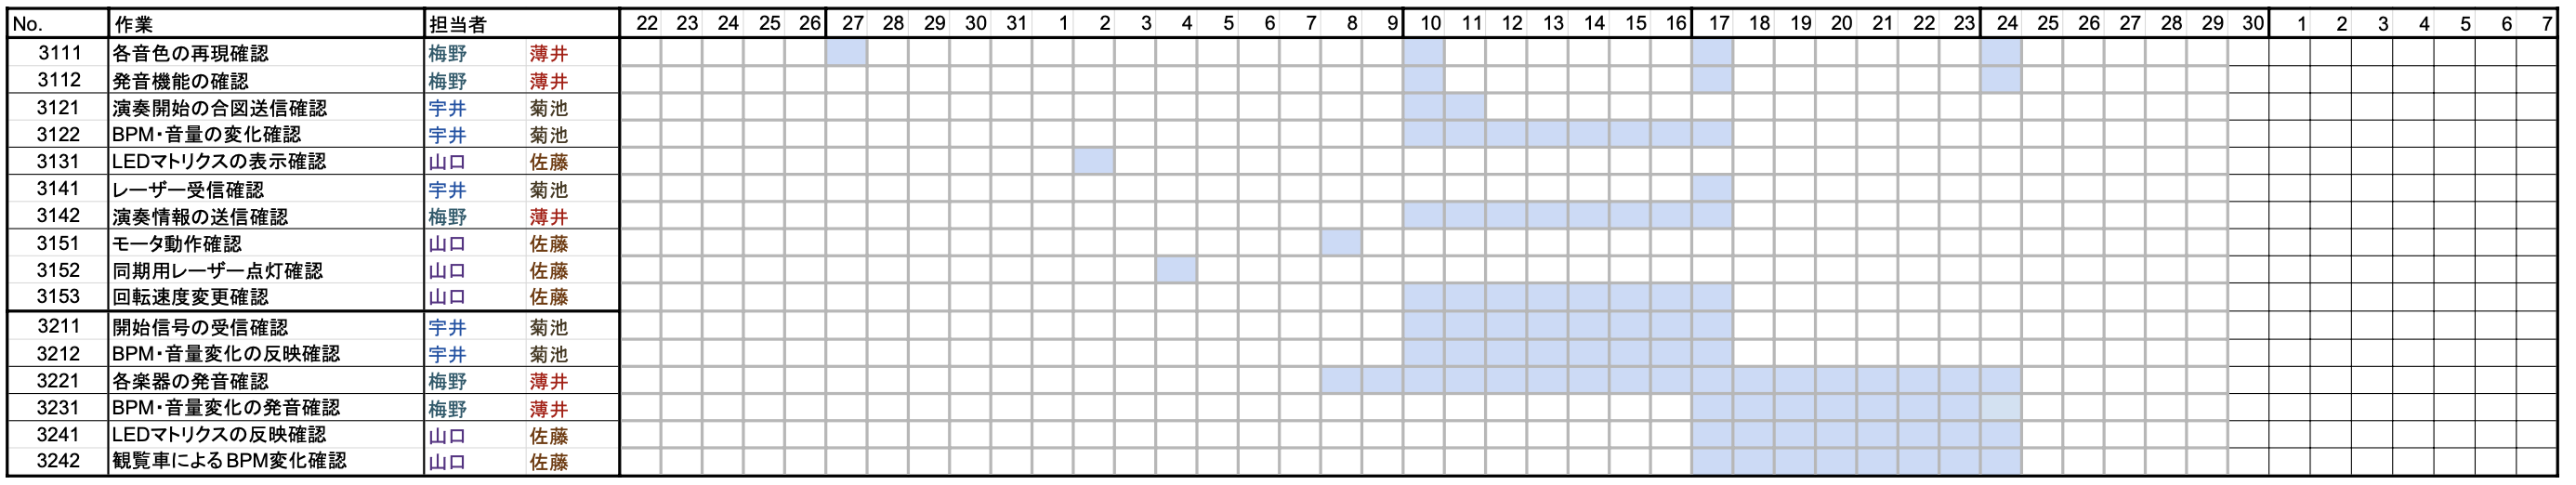
\includegraphics[width=0.9\columnwidth]{gant8.png}
    \caption{現在のガントチャート（テストフェーズ）}
    \label{fig:gant8}
\end{figure}


\sectionrule


\section{課題管理}

\begin{tabularx}{\linewidth}{@{}p{3cm}Xllp{3.2cm}ll@{}}
\toprule
課題 & 発生原因 & 影響度 & 優先度 & 対策 & 期限 & 状態 \\
\midrule
可変抵抗器がブレッドボード上で安定接続できない（No.2112/2113に影響） & スライド式可変抵抗器の端子形状がブレッドボードに適合しないため． & 高 & 高 & スライド式可変抵抗器を基盤に設置し，筐体へ固定した． & 6/12 & 対応済 \\
\midrule
1機のスライド式可変抵抗器のはんだ付け設置不良（No.2112に影響） & 基盤へのはんだ付け時に接触不良が発生したため． & 中 & 高 & 6/10に再はんだ付けを実施し，動作を確認した． & 6/10 & 対応済 \\
\bottomrule
\end{tabularx}

\medskip
※影響度＝プロジェクトへのインパクト

※優先度＝対応の緊急性

\sectionrule


\section{AI利用状況と検証（再現性重視）}

\subsection{利用内容}

\begin{itemize}
  \item 利用目的：設計・実装支援・レビュー

  \item 入力（プロンプト要旨）：
    \begin{itemize}
      \item タクトスイッチ（ボタン）の動作確認用プログラム（button\_test）の
      作成方法について質問した．

      \item 段ボール筐体へ基盤・センサ類を固定する際の，
      配線整理や配置の方針について質問した．
    \end{itemize}

  \item 出力概要：
    \begin{itemize}
      \item タクトスイッチの押下をデバッグ出力で確認する
      検証用プログラムの実装方法の説明が得られた．

      \item センサ・基盤を筐体内に固定する際の，
      配線取り回しと操作部配置の方針が得られた．
    \end{itemize}
\end{itemize}


\sectionrule

\subsection{検証方法}

\begin{itemize}

    \item 検証手法：
      \begin{itemize}
        \item AIが生成したタクトスイッチ動作確認プログラムをArduino IDE上で
        コンパイル・実行し，押下に応じてシリアルモニタの出力が変化するか確認した．

        \item AIの出力内容とArduino公式ドキュメントを比較し，
        使用関数や実装方法に誤りがないか確認した．
      \end{itemize}

      \item 参照資料：
      \begin{itemize}
        \item Arduino公式ドキュメント：
        \url{https://docs.arduino.cc/}

        \item Arduino Tutorials：
        \url{https://docs.arduino.cc/tutorials/}
      \end{itemize}

      \item 検証手順：
    \begin{enumerate}
      \item AIへタクトスイッチの動作確認方法について質問した．

      \item AIが生成した内容をもとに検証用プログラムを作成した．

      \item Arduinoへプログラムを書き込み，
      シリアルモニタおよび実機で動作を確認した．

      \item AIの出力内容をArduino公式ドキュメントと比較し，
      実装内容に誤りがないことを確認した．
    \end{enumerate}

\end{itemize}


\sectionrule

\subsection{ファクトチェック結果}


\begin{itemize}

    \item 一致点：
      \begin{itemize}
        \item AIが提示したタクトスイッチの読み取り処理は，
        Arduino公式ドキュメントの内容と一致していた．
      \end{itemize}

      \item 不一致・疑義：
    \begin{itemize}
      \item 一部のサンプルコードにおいて，
      プルアップ／プルダウンの設定が実際の配線と異なる場合があり，
      修正が必要であった．
    \end{itemize}

  \item 最終判断：
    \begin{itemize}
      \item 一部採用
    \end{itemize}

    \item 根拠：
    \begin{itemize}
      \item Arduino公式ドキュメントとの比較により，
      AIの出力内容がおおむね正確であることを確認したため．

      \item 実際に検証用プログラムを動作させ，
      正常に動作することを確認したため．
    \end{itemize}

\end{itemize}


\sectionrule


\section{次回計画}


\begin{itemize}

  \item 目標：指揮デバイスの完成（筐体の最終固定），観覧車型中継機の製作着手
    \begin{itemize}
      \item 指揮デバイスの筐体を最終固定し，
      本体・センサの実装を完了する．

      \item 観覧車型中継機の部品用意および本体製作に着手する．
    \end{itemize}

  \item 達成基準：
    \begin{itemize}
      \item 指揮デバイスの筐体が完成し，各操作部が正しく動作すること．

      \item 観覧車型中継機の部品が用意され，製作に着手できていること．
    \end{itemize}

  \item 期限：
    \begin{itemize}
      \item 2026/6/23
    \end{itemize}

\end{itemize}


\sectionrule


\section{その他}

\begin{itemize}
  \item {}指揮デバイスの筐体は，計画書および第六回で想定した3Dプリンタ製（Tinkercad設計）から段ボール製に変更しており，今回その制作がほぼ完成した．
\end{itemize}

\sectionrule


\section{付録}

\begin{itemize}
  \item 添付資料：
    \begin{itemize}
      \item No.2112(タクトスイッチの動作確認)のプログラム：\url{https://github.com/Sato907/3S_HCK1/tree/main/HCK1_group/HCK1_group_mywork/button_test}
      \item No.2113(可変抵抗器から読み取った値を5段階にして出力するプログラム)のプログラム：\url{https://github.com/Sato907/3S_HCK1/tree/main/HCK1_group/HCK1_group_mywork/shiki_device}

    \end{itemize}

\end{itemize}

\sectionrule

\end{document}
